\documentclass[12pt,a4paper]{article}
\usepackage{amsmath,amscd,amsbsy,amssymb,latexsym,url,bm,amsthm}
\usepackage{epsfig,graphicx,subfigure}
\usepackage{enumitem,balance}
\usepackage{wrapfig}
\usepackage{mathrsfs,euscript}
\usepackage[usenames]{xcolor}
\usepackage{hyperref}
\usepackage[vlined,ruled,linesnumbered]{algorithm2e}
\hypersetup{colorlinks=true,linkcolor=black}

\newtheorem{theorem}{Theorem}
\newtheorem{lemma}[theorem]{Lemma}
\newtheorem{proposition}[theorem]{Proposition}
\newtheorem{corollary}[theorem]{Corollary}
\newtheorem{exercise}{Exercise}
\newtheorem*{solution}{Solution}
\newtheorem{definition}{Definition}
\theoremstyle{definition}

\renewcommand{\thefootnote}{\fnsymbol{footnote}}

\newcommand{\postscript}[2]
 {\setlength{\epsfxsize}{#2\hsize}
  \centerline{\epsfbox{#1}}}

\renewcommand{\baselinestretch}{1.0}

\setlength{\oddsidemargin}{-0.365in}
\setlength{\evensidemargin}{-0.365in}
\setlength{\topmargin}{-0.3in}
\setlength{\headheight}{0in}
\setlength{\headsep}{0in}
\setlength{\textheight}{10.1in}
\setlength{\textwidth}{7in}
\makeatletter \renewenvironment{proof}[1][Proof] {\par\pushQED{\qed}\normalfont\topsep6\p@\@plus6\p@\relax\trivlist\item[\hskip\labelsep\bfseries#1\@addpunct{.}]\ignorespaces}{\popQED\endtrivlist\@endpefalse} \makeatother
\makeatletter
\renewenvironment{solution}[1][Solution] {\par\pushQED{\qed}\normalfont\topsep6\p@\@plus6\p@\relax\trivlist\item[\hskip\labelsep\bfseries#1\@addpunct{.}]\ignorespaces}{\popQED\endtrivlist\@endpefalse} \makeatother

\begin{document}
\noindent

%========================================================================
\noindent\framebox[\linewidth]{\shortstack[c]{
\Large{\textbf{Lab03-Matroid \& Dynamic Programming}}\vspace{1mm}\\
CS2308-Algorithm and Complexity, Xiaofeng Gao, Spring 2022.}}
\begin{center}
\footnotesize{\color{red}$*$ If there is any problem, please contact TA Hongjie Fang.}

% Please write down your name, student id and email.
\footnotesize{\color{blue}$*$ Name: Zhenran Xiao  \quad Student ID: 520030910281 \quad Email: xiaozhenran@sjtu.edu.cn}
\end{center}

\begin{enumerate}
	\item Let $S$ be a finite set and let $S_1, S_2, \cdots, S_n$ be a partition of $S$ into non-empty disjoint subsets. Define structure $(S, \mathcal{I})$ by the condition that 
	$$
	\mathcal{I} = \{I \mid I \subseteq S, \left|I \cap S_i \right| \leq k_i \textrm{ for } i=1,2,\cdots,n\}
	$$
	where $k_1, k_2, \cdots, k_n$ are positive integers. Does $(S, \mathcal{I})$ form a matroid? Why or why not? (\textit{\color{blue}Hint: you may start from a simple case that $k_1 = k_2 = \cdots = k_n = 1$.})
	
	    \begin{solution}
	    	\quad \\
	    	$(S, \mathcal{I})$ form a matroid. Proof is following. \\
	    	\quad \\
	        Hereditary: \\
	        If A $\subset$ B and B $\in$ $\mathcal{I}$, meaning
	        $$
	        B \subseteq S, \left|B \cap S_i \right| \leq k_i \textrm{ for } i=1,2,\cdots,n\
	        $$
	        Obviously, 
	        $$
	        A \subseteq S, \left|A \cap S_i \right| \leq k_i \textrm{ for } i=1,2,\cdots,n\
	        $$
	        Namely, A $\in$ $\mathcal{I}$. \\
	        \quad \\
	        Exchange Property: \\
	        Assume that $k_1 = k_2 = \cdots = k_n = 1$, so we can easily know set $I$ is composed of each one or zero element selected from $S_1, S_2, \cdots, S_n$. If A, B $\in$ $\mathcal{I}$, |A|<|B|, there must exists an $S_p$ that B has an element $x$ selected from it but A doesn't have. Namely $x \in B\backslash A$. We create set $M = A \cup \{x\}$. Before, $\left|A \cap S_p \right| = 0$, now, $\left|M \cap S_p \right| = 1 \leq k_p$. For other $S_i$, $M$ is the same as $A$. So 
	        $$
	        M \subseteq S, \left|M \cap S_i \right| \leq k_i \textrm{ for } i=1,2,\cdots,n\
	        $$
	        Namely, $A \cup \{x\} \in \mathcal{I}$. \\
	        If $k_i$ are bigger, the proof is in a similar way.
	    \end{solution}
	
	\item Given $n$ matrices $A_1, A_2, \cdots, A_n$ and $(n+1)$ positive integers $m_1, m_2, \cdots, m_{n+1}$. The $i$-th matrix $A_i$ $(1 \leq i \leq n)$ has the size of $m_i \times m_{i+1}$. Our goal is to calculate $A_1\times A_2\times \cdots \times A_n$. For any two matrix $P_{p\times q}$ and $Q_{q\times r}$, the computational cost of $P\times Q$ is $p\cdot q\cdot r$. Due to the combination law of matrix multiplication, we can arbitrarily add parentheses to change the calculation order without changing the final result. Since different methods of adding parentheses have different computational costs, please design an algorithm to minimize the total computational costs. You need to briefly describe your algorithm and write it in pseudo-code, then analyze the time complexity and space complexity of your algorithm.
	
	\textbf{Example}. $A_1$ is a $4 \times 2$ matrix, $A_2$ is a $2\times 3$ matrix, $A_3$ is a $3 \times 1$ matrix. If we calculate $A_1\times A_2\times A_3$ as the original order, the total computational costs are $4\times 2\times 3 + 4\times 3\times 1 = 36$. But if we calculate it as $A_1 \times (A_2 \times A_3)$, the total computational costs are $2\times 3 \times 1 + 4 \times 2 \times 1 = 14$. In this example, your algorithm should output the minimum total computational cost $14$.

	    \begin{solution}
	        \quad \\
	        Let $c[i,j]$ be the minimum cost computing $A_iA_{i+1}\cdots Aj$, then we get the recursive formula
	        $$
	        c[i,j] = \left\{
	        \begin{aligned}
	        	& 0 & i = j \\
	        	& min\{c[i,k] + c[k+1,j] + m_{i-1}m_km_j\} & i<j
	        \end{aligned}
	        \right.
	        $$
	        For every $k$ from $i$ to $j-1$, calculate the cost and find the minimum situation.\\
	        In the algorithm, 
	        $c[1,\cdots,n,1,\cdots,n]$ stores the cost $c[i,j]$;  $s[1,\cdots,n,2,\cdots,n]$ records the segmentation point $k$ corresponding to the optimal cost $c[i,j]$. \\
	        \begin{algorithm}[H]
	        	\KwIn{array[$m_1,...,m_{n+1}$]}
	        	\KwOut{computational cost, an interger}
	        	\BlankLine
	        	\caption{$minCost(array[m_1,...,m_{n+1}])$} \label{Alg-div}
	        	Let $c[1,\cdots,n,1,\cdots,n]$ and $s[1,\cdots,n,2,\cdots,n]$ be new tables\;
	        	\For{i $\leftarrow$ 1 to n}
	        	{
	        		$c[i,i] = 0$\;
	        	}
        		\For{l $\leftarrow$ 2 to n}
        		{
        			\For{i $\leftarrow$ 1 to n-l+1}
        			{
        				$j = i+l-1$\;
        				$c[i,j] = \infty$\;
        				\For{k $\leftarrow$ i to j-1}
        				{
        					$q = c[i,k]+c[k+1,j]+m_{i-1}m_km_j$\;
        					\If{q < c[i,j]}
        					{
        						$c[i,j] = q$\;
        						$s[i,j] = k$\;
        					}
        				}
        			}
        		}
	        	\Return{c[1,n]}\;      	
	        \end{algorithm}
        The time complexity is 
        \[
        	T(n) = n + (n-1)^3 \sim O(n^3)
        \]
        The space complexity is 
        \[
        	S(n) = n^2 + n(n-1) \sim O(n^2)
        \]
	    \end{solution}
	
	\item You are given an $m \times n$ matrix $A$ with integer elements. Initially, you are located at the top-left corner $(1, 1)$, and in each step, you can only move right or down in the matrix. Among all possible paths starting from the top-left corner $(1, 1)$ and ending in the bottom-right corner $(m, n)$, find the path with the maximum non-negative product. The product of a path is the product of all integers in the grid cells visited along the path.
	\begin{enumerate}
		\item If all elements in $A$ are non-negative integers, design an algorithm to solve the problem. Your algorithm should return the maximum non-negative product as well as the optimal path. Write the algorithm in pseudo-code and analyze its time complexity.
		\item If the elements in $A$ are arbitrary integers, design an algorithm to solve the problem. Your algorithm should return the maximum non-negative product. Specially, if the maximum product is negative, your algorithm should return $-1$. Briefly describe your algorithm and analyze its time complexity.
	\end{enumerate}

	\textbf{Example}. An example of the problem is illustrated in Fig. \ref{Fig-P3Example}. The path marked in blue is the optimal path, whose product is $1\times 1\times (-2)\times (-4)\times 1 = 8$.
	
	\begin{figure}[h]
		\centering
		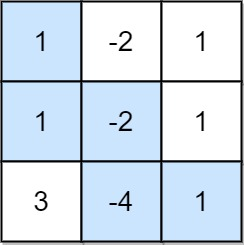
\includegraphics[width=1in]{Fig-P3Example.jpeg}
		\caption{An Example of the Maximum Non-negative Product Path Problem}\label{Fig-P3Example}
	\end{figure}
	
	\newpage
	    \begin{solution}
	        \quad \\
	        (a)\\
	        Let $maxp[i,j]$ be the maximun product moving to $A[i,j]$, then we get the recursive formula
	        $$
	        maxp[i,j] = \left\{
	        \begin{aligned}
	        	& A[1,1] & i = 1, j = 1 \\
	        	& maxp[i,j-1] \times A[i,j] & i = 1, j\neq 1 \\
	        	& maxp[i-1,j] \times A[i,j] & i\neq 1, j = 1 \\
	        	& max(maxp[i,j-1],maxp[i-1,j]) \times A[i,j] & i\neq 1, j\neq 1
	        \end{aligned}
	        \right.
	        $$
	        In the algorithm, 
	        $maxp[1,\cdots ,m,1,\cdots ,n]$ stores the maximum product $maxp[i,j]$;  $path[1,\cdots ,m,1,\cdots ,n]$ records the path. \\
	        \begin{algorithm}[H]
	        	\KwIn{an m$\times$ n matrix A with non-negative integer elements.}
	        	\KwOut{the maximum non-negative product and the optimal path}
	        	\BlankLine
	        	\caption{$optPath\_nn(A_{m\times n})$} \label{Alg-div}
	        	Let $maxp[1,\cdots,m,1,\cdots,n]$ and $path[1,\cdots,m,1,\cdots,n]$ be new tables\;
	        	$maxp[1][1]\leftarrow A[1,1]$\; 
	        	\For{j$\leftarrow$ 2 to n}
	        	{
	        		$maxp[1][j] \leftarrow maxp[1][j-1]\times A[1,j]$\;  
	        	}
        		\For{i$\leftarrow$ 2 to m}
        		{
        			$maxp[i][1] \leftarrow maxp[i-1][1]\times A[j,1]$\;  
        		}
        		\For{i$\leftarrow$ 2 to m}
        		{
        			\For{j$\leftarrow$ 2 to n}
        			{
        				$maxp[i,j] \leftarrow max(maxp[i,j-1],maxp[i-1,j]) \times A[i,j]$\;
        				\If{maxp[i,j-1] > maxp[i-1,j]}
        				{
        					$path[i, j-1] \leftarrow$ ``$\rightarrow$"\; 
        				}
        				\ElseIf{maxp[i,j-1] < maxp[i-1,j]}
        				{
        					$path[i-1, j] \leftarrow$ ``$\downarrow$"\; 
        				}
        				\Else
        				{
        					$path[i, j-1] \leftarrow$ ``$\rightarrow$"\; 
        					$path[i-1, j] \leftarrow$ ``$\downarrow$"\; 
        				}
        			}
        		}
	        	\Return{$maxp[m,n]$ and $path[1,\cdots,m,1,\cdots,n]$}\;
	        \end{algorithm}
        	The time complexity is 
        	\[
        	T(n) = m + n + (m-1)(n-1) \sim O(mn)
        	\]
        	The space complexity is 
        	\[
        	S(n) = mn + mn \sim O(mn)
        	\]
        	\newpage
        	(b) \\
        	Since there are positive and negative elements in the matrix, in order to obtain the maximum product, we shouldn't only store the maximum product in the process of moving. For example, if the current element is negative, the left is negative, the upper is positive, the upper is larger than the left, but obviously the left can make the product larger. Therefore, we need to store both the minimum and maximum of the product as it moves.
        	 \begin{algorithm}[H]
        	 	\KwIn{an m$\times$ n matrix A with integer elements.}
        	 	\KwOut{the maximum non-negative product and the optimal path}
        	 	\BlankLine
        	 	\caption{$optPath(A_{m\times n})$} \label{Alg-div}
        	 	Let $maxp[1,\cdots,m,1,\cdots,n]$, $minp[1,\cdots,m,1,\cdots,n]$ and $path[1,\cdots,m,1,\cdots,n]$ be new tables\;
        	 	$maxp[1][1]\leftarrow A[1,1]$\; 
        	 	$minp[1][1]\leftarrow A[1,1]$\; 
        	 	\For{j$\leftarrow$ 2 to n}
        	 	{
        	 		$maxp[1][j] \leftarrow maxp[1][j-1]\times A[1,j]$\;
        	 		$minp[1][j] \leftarrow minp[1][j-1]\times A[1,j]$\;  
        	 	}
        	 	\For{i$\leftarrow$ 2 to m}
        	 	{
        	 		$maxp[i][1] \leftarrow maxp[i-1][1]\times A[j,1]$\;  
        	 		$minp[i][1] \leftarrow minp[i-1][1]\times A[j,1]$\;  
        	 	}
        	 	\For{i$\leftarrow$ 2 to m}
        	 	{
        	 		\For{j$\leftarrow$ 2 to n}
        	 		{
        	 			\If{A[i][j] >= 0}
        	 			{
        	 				$maxp[i,j] \leftarrow max(maxp[i,j-1],maxp[i-1,j]) \times A[i,j]$\;
        	 				$minp[i,j] \leftarrow min(minp[i,j-1],minp[i-1,j]) \times A[i,j]$\;
        	 				\If{maxp[i,j-1] > maxp[i-1,j]}
        	 				{
        	 					$path[i, j-1] \leftarrow$ ``$\rightarrow$"\; 
        	 				}
        	 				\ElseIf{maxp[i,j-1] < maxp[i-1,j]}
        	 				{
        	 					$path[i-1, j] \leftarrow$ ``$\downarrow$"\; 
        	 				}
        	 				\Else
        	 				{
        	 					$path[i, j-1] \leftarrow$ ``$\rightarrow$"\; 
        	 					$path[i-1, j] \leftarrow$ ``$\downarrow$"\; 
        	 				}
        	 			}
         				\Else
         				{
         					$maxp[i,j] \leftarrow min(minp[i,j-1],minp[i-1,j]) \times A[i,j]$\;
         					$minp[i,j] \leftarrow max(maxp[i,j-1],maxp[i-1,j]) \times A[i,j]$\;
         					\If{minp[i,j-1] < minp[i-1,j]}
         					{
         						$path[i, j-1] \leftarrow$ ``$\rightarrow$"\; 
         					}
         					\ElseIf{minp[i,j-1] > minp[i-1,j]}
         					{
         						$path[i-1, j] \leftarrow$ ``$\downarrow$"\; 
         					}
         					\Else
         					{
         						$path[i, j-1] \leftarrow$ ``$\rightarrow$"\; 
         						$path[i-1, j] \leftarrow$ ``$\downarrow$"\; 
         					}
         				}
        	 		}
        	 	}
         		\If{maxp[m,n] < 0}
         		{
         			\Return{-1}
         		}
         		\Else
         		{
         			\Return{$maxp[m,n]$ and $path[1,\cdots,m,1,\cdots,n]$}\;
         		}
        	 \end{algorithm}
         	The time complexity is 
         	\[
         	T(n) = m + n + (m-1)(n-1) \sim O(mn)
         	\]
         	The space complexity is 
         	\[
         	S(n) = 2mn + mn \sim O(mn)
         	\]
	    \end{solution}

\end{enumerate}

\vspace{20pt}

\textbf{Remark:} You need to include your .pdf and .tex files in your uploaded .rar or .zip file.

%========================================================================
\end{document}
